\documentclass[twoside]{book}

% Packages required by doxygen
\usepackage{calc}
\usepackage{doxygen}
\usepackage{graphicx}
\usepackage[utf8]{inputenc}
\usepackage{makeidx}
\usepackage{multicol}
\usepackage{multirow}
\usepackage{textcomp}
\usepackage[table]{xcolor}

% Font selection
\usepackage[T1]{fontenc}
\usepackage{mathptmx}
\usepackage[scaled=.90]{helvet}
\usepackage{courier}
\usepackage{amssymb}
\usepackage{sectsty}
\renewcommand{\familydefault}{\sfdefault}
\allsectionsfont{%
  \fontseries{bc}\selectfont%
  \color{darkgray}%
}
\renewcommand{\DoxyLabelFont}{%
  \fontseries{bc}\selectfont%
  \color{darkgray}%
}

% Page & text layout
\usepackage{geometry}
\geometry{%
  a4paper,%
  top=2.5cm,%
  bottom=2.5cm,%
  left=2.5cm,%
  right=2.5cm%
}
\tolerance=750
\hfuzz=15pt
\hbadness=750
\setlength{\emergencystretch}{15pt}
\setlength{\parindent}{0cm}
\setlength{\parskip}{0.2cm}
\makeatletter
\renewcommand{\paragraph}{%
  \@startsection{paragraph}{4}{0ex}{-1.0ex}{1.0ex}{%
    \normalfont\normalsize\bfseries\SS@parafont%
  }%
}
\renewcommand{\subparagraph}{%
  \@startsection{subparagraph}{5}{0ex}{-1.0ex}{1.0ex}{%
    \normalfont\normalsize\bfseries\SS@subparafont%
  }%
}
\makeatother

% Headers & footers
\usepackage{fancyhdr}
\pagestyle{fancyplain}
\fancyhead[LE]{\fancyplain{}{\bfseries\thepage}}
\fancyhead[CE]{\fancyplain{}{}}
\fancyhead[RE]{\fancyplain{}{\bfseries\leftmark}}
\fancyhead[LO]{\fancyplain{}{\bfseries\rightmark}}
\fancyhead[CO]{\fancyplain{}{}}
\fancyhead[RO]{\fancyplain{}{\bfseries\thepage}}
\fancyfoot[LE]{\fancyplain{}{}}
\fancyfoot[CE]{\fancyplain{}{}}
\fancyfoot[RE]{\fancyplain{}{\bfseries\scriptsize Generated on Tue Jun 10 2014 14\-:54\-:07 for Open\-C\-L for J\-T\-C by Doxygen }}
\fancyfoot[LO]{\fancyplain{}{\bfseries\scriptsize Generated on Tue Jun 10 2014 14\-:54\-:07 for Open\-C\-L for J\-T\-C by Doxygen }}
\fancyfoot[CO]{\fancyplain{}{}}
\fancyfoot[RO]{\fancyplain{}{}}
\renewcommand{\footrulewidth}{0.4pt}
\renewcommand{\chaptermark}[1]{%
  \markboth{#1}{}%
}
\renewcommand{\sectionmark}[1]{%
  \markright{\thesection\ #1}%
}

% Indices & bibliography
\usepackage{natbib}
\usepackage[titles]{tocloft}
\setcounter{tocdepth}{3}
\setcounter{secnumdepth}{5}
\makeindex

% Hyperlinks (required, but should be loaded last)
\usepackage{ifpdf}
\ifpdf
  \usepackage[pdftex,pagebackref=true]{hyperref}
\else
  \usepackage[ps2pdf,pagebackref=true]{hyperref}
\fi
\hypersetup{%
  colorlinks=true,%
  linkcolor=blue,%
  citecolor=blue,%
  unicode%
}

% Custom commands
\newcommand{\clearemptydoublepage}{%
  \newpage{\pagestyle{empty}\cleardoublepage}%
}


%===== C O N T E N T S =====

\begin{document}

% Titlepage & ToC
\hypersetup{pageanchor=false}
\pagenumbering{roman}
\begin{titlepage}
\vspace*{7cm}
\begin{center}%
{\Large Open\-C\-L for J\-T\-C \\[1ex]\large 0.\-1 }\\
\vspace*{1cm}
{\large Generated by Doxygen 1.8.6}\\
\vspace*{0.5cm}
{\small Tue Jun 10 2014 14:54:07}\\
\end{center}
\end{titlepage}
\clearemptydoublepage
\tableofcontents
\clearemptydoublepage
\pagenumbering{arabic}
\hypersetup{pageanchor=true}

%--- Begin generated contents ---
\chapter{Main Page}
\label{index}\hypertarget{index}{}This is the Open\-C\-L version of J\-T\-C extra stuff \hypertarget{index_Introduction}{}\section{Introduction}\label{index_Introduction}
The rapid development of parallel hardware in the last decade requires a constant evaluation of the parallel algoritms used in large scale scientific applications . Iterative kernels are essential components of iterative solvers which are the preferred technique in a variety of large scale problems. Jacobi iteration for the second order discretisation of the Laplacian $ 3D$ operator\-: \begin{equation} u^{(new)}_{i,j,k}=\frac{1}{6}(u^{(old)}_{i-1,j,k}+ u^{(old)}_{i+1,j,k}+u^{(old)}_{i,j-1,k}+ u^{(old)}_{i,j+1,k}+u^{(old)}_{i,j,k-1}+u^{(old)}_{i,j,k+1}) \ , \end{equation} is the one of the simplest, yet not trivial, example of iterative kernel. In its simple form it contains the features relevant to the performance for a large class of iterators\-: i) stranded memory access and ii) low number of floating point operations per memory reference. \hypertarget{index_Results}{}\section{Results}\label{index_Results}

\begin{DoxyImage}
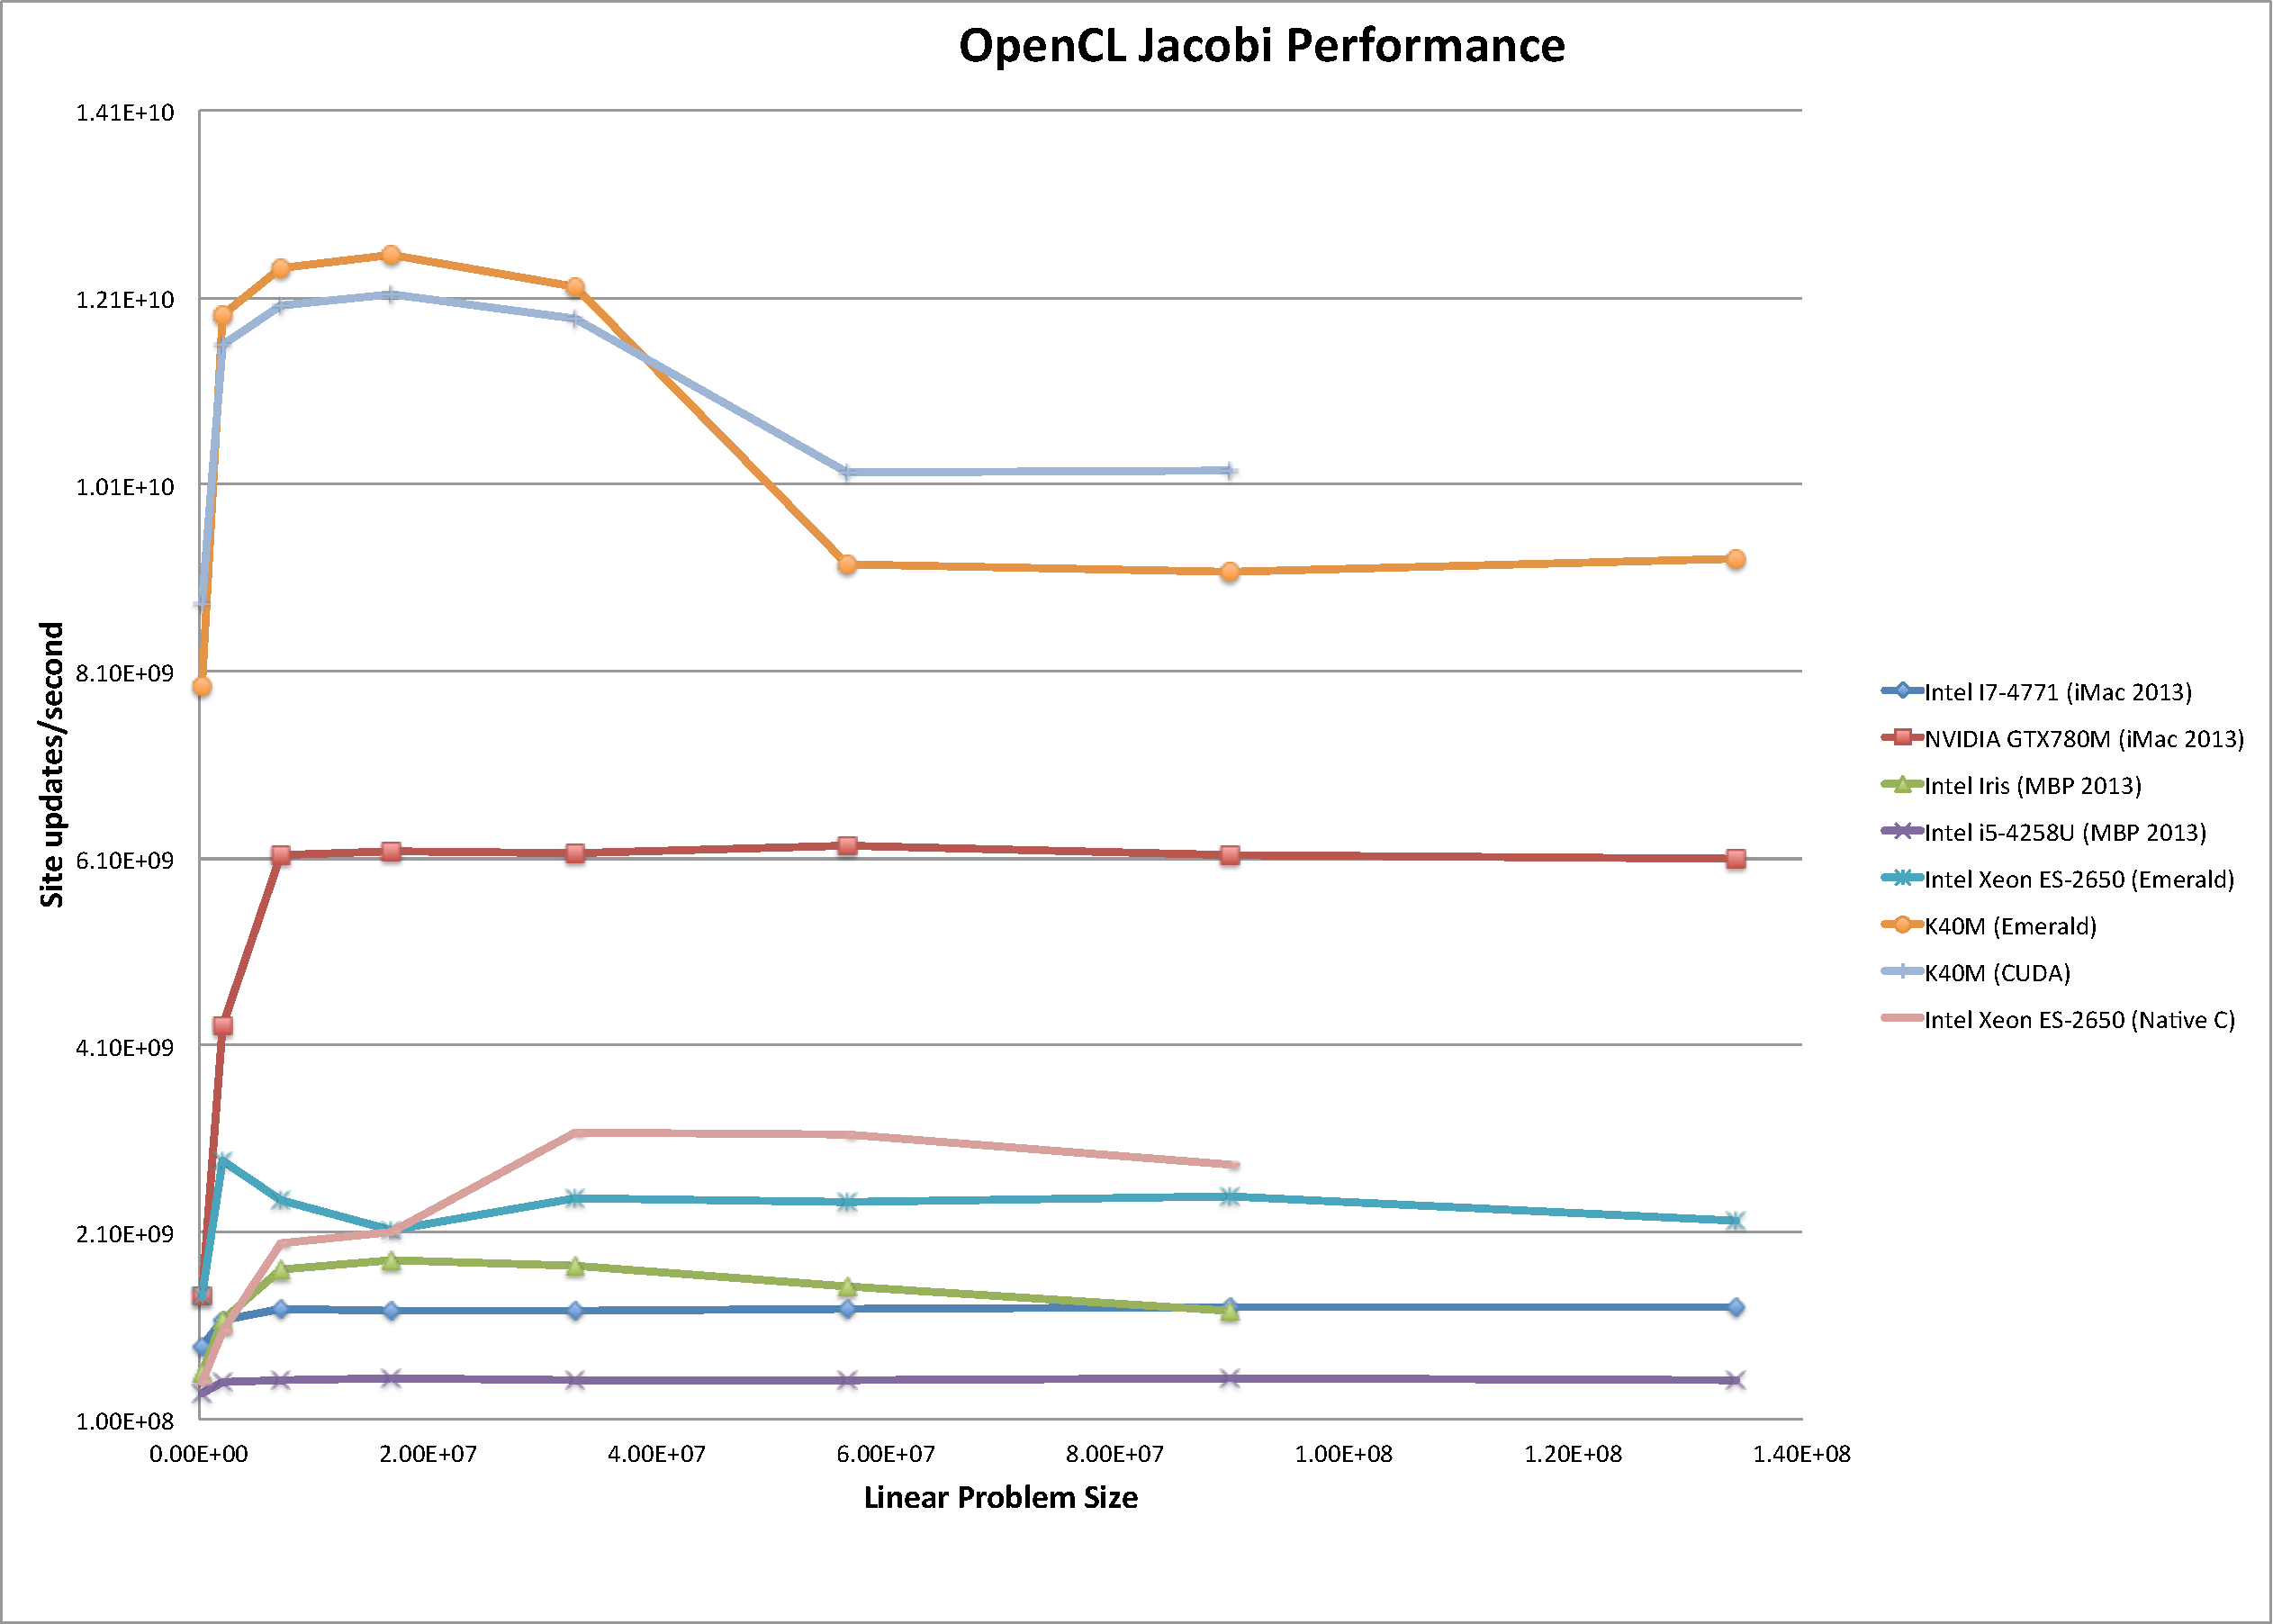
\includegraphics[width=10cm]{OPENCLRESULTS}
\caption{My application}
\end{DoxyImage}
 
\chapter{Todo List}
\label{todo}
\hypertarget{todo}{}

\begin{DoxyRefList}
\item[\label{todo__todo000003}%
\hypertarget{todo__todo000003}{}%
File \hyperlink{jacobi__opencl_8h}{jacobi\-\_\-opencl.h} ]Include header files to grab typename Real  
\item[\label{todo__todo000004}%
\hypertarget{todo__todo000004}{}%
File \hyperlink{jacobi__relaxation__ocl_8cl}{jacobi\-\_\-relaxation\-\_\-ocl.cl} ]include the header to grab the typedef of Real  
\item[\label{todo__todo000001}%
\hypertarget{todo__todo000001}{}%
Global \hyperlink{jacobi__opencl_8h_a4bc101c6eca787275f55ca9cc0d437a7}{Open\-C\-L\-\_\-\-Jacobi} (int Nx, int Ny, int Nx, Real $\ast$unknown)]modify prototype to pass in opencl struct  
\item[\label{todo__todo000002}%
\hypertarget{todo__todo000002}{}%
Global \hyperlink{jacobi__opencl_8h_ae84f123b51a423b6415eb98e21310846}{Open\-C\-L\-\_\-\-Jacobi\-\_\-\-Iteration} (int max\-Iters, int convergence\-Iters)]Fix this memory transfer 
\end{DoxyRefList}
\chapter{Data Structure Index}
\section{Data Structures}
Here are the data structures with brief descriptions\-:\begin{DoxyCompactList}
\item\contentsline{section}{\hyperlink{struct_open_c_l_instance}{Open\-C\-L\-Instance} }{\pageref{struct_open_c_l_instance}}{}
\end{DoxyCompactList}

\chapter{File Index}
\section{File List}
Here is a list of all files with brief descriptions\-:\begin{DoxyCompactList}
\item\contentsline{section}{\hyperlink{jacobi__opencl_8c}{jacobi\-\_\-opencl.\-c} }{\pageref{jacobi__opencl_8c}}{}
\item\contentsline{section}{\hyperlink{jacobi__opencl_8h}{jacobi\-\_\-opencl.\-h} }{\pageref{jacobi__opencl_8h}}{}
\item\contentsline{section}{\hyperlink{jacobi__relaxation__ocl_8cl}{jacobi\-\_\-relaxation\-\_\-ocl.\-cl} }{\pageref{jacobi__relaxation__ocl_8cl}}{}
\end{DoxyCompactList}

\chapter{Data Structure Documentation}
\hypertarget{struct_open_c_l_instance}{\section{Open\-C\-L\-Instance Struct Reference}
\label{struct_open_c_l_instance}\index{Open\-C\-L\-Instance@{Open\-C\-L\-Instance}}
}


{\ttfamily \#include $<$jacobi\-\_\-opencl.\-h$>$}

\subsection*{Data Fields}
\begin{DoxyCompactItemize}
\item 
cl\-\_\-device\-\_\-id \hyperlink{struct_open_c_l_instance_a22e36a6758529a5000288a7dfb5fd231}{device\-\_\-id}
\item 
cl\-\_\-context \hyperlink{struct_open_c_l_instance_a44eab7fed94fa64d0a67fa3f992ce502}{context}
\item 
cl\-\_\-command\-\_\-queue \hyperlink{struct_open_c_l_instance_a0af493bf8b0fa33e91dd7e7675b4a2d8}{commands}
\item 
cl\-\_\-program \hyperlink{struct_open_c_l_instance_a883163fd9246e6704b1334e69548158c}{program}
\item 
cl\-\_\-kernel \hyperlink{struct_open_c_l_instance_ac97210abd5948c1c67da9a0f7fa6f646}{jacobi\-\_\-ocl}
\item 
cl\-\_\-mem \hyperlink{struct_open_c_l_instance_ae2de6de8249187081eab1b552ba1c1a0}{d\-\_\-u1}
\item 
cl\-\_\-mem \hyperlink{struct_open_c_l_instance_a1625f6746ccb378443e0195e74c99f9a}{d\-\_\-u2}
\item 
unsigned int \hyperlink{struct_open_c_l_instance_a19687918b1afb192ab716e277960738f}{x\-Dim}
\item 
unsigned int \hyperlink{struct_open_c_l_instance_a05ee9f97ea7397d010948c5f13e85529}{y\-Dim}
\item 
unsigned int \hyperlink{struct_open_c_l_instance_a20e097a486b0f9b58dbd53b97f09e26c}{z\-Dim}
\end{DoxyCompactItemize}


\subsection{Detailed Description}
\hyperlink{struct_open_c_l_instance}{Open\-C\-L\-Instance} -\/ A struct containing the device ide, context, command queue, program, kernel and problem size for Open\-C\-L 

Definition at line 37 of file jacobi\-\_\-opencl.\-h.



\subsection{Field Documentation}
\hypertarget{struct_open_c_l_instance_a0af493bf8b0fa33e91dd7e7675b4a2d8}{\index{Open\-C\-L\-Instance@{Open\-C\-L\-Instance}!commands@{commands}}
\index{commands@{commands}!OpenCLInstance@{Open\-C\-L\-Instance}}
\subsubsection[{commands}]{\setlength{\rightskip}{0pt plus 5cm}cl\-\_\-command\-\_\-queue Open\-C\-L\-Instance\-::commands}}\label{struct_open_c_l_instance_a0af493bf8b0fa33e91dd7e7675b4a2d8}
Compute command queue 

Definition at line 40 of file jacobi\-\_\-opencl.\-h.

\hypertarget{struct_open_c_l_instance_a44eab7fed94fa64d0a67fa3f992ce502}{\index{Open\-C\-L\-Instance@{Open\-C\-L\-Instance}!context@{context}}
\index{context@{context}!OpenCLInstance@{Open\-C\-L\-Instance}}
\subsubsection[{context}]{\setlength{\rightskip}{0pt plus 5cm}cl\-\_\-context Open\-C\-L\-Instance\-::context}}\label{struct_open_c_l_instance_a44eab7fed94fa64d0a67fa3f992ce502}
Compute context 

Definition at line 39 of file jacobi\-\_\-opencl.\-h.

\hypertarget{struct_open_c_l_instance_ae2de6de8249187081eab1b552ba1c1a0}{\index{Open\-C\-L\-Instance@{Open\-C\-L\-Instance}!d\-\_\-u1@{d\-\_\-u1}}
\index{d\-\_\-u1@{d\-\_\-u1}!OpenCLInstance@{Open\-C\-L\-Instance}}
\subsubsection[{d\-\_\-u1}]{\setlength{\rightskip}{0pt plus 5cm}cl\-\_\-mem Open\-C\-L\-Instance\-::d\-\_\-u1}}\label{struct_open_c_l_instance_ae2de6de8249187081eab1b552ba1c1a0}
Device memory used for the input unknown 1 vector 

Definition at line 44 of file jacobi\-\_\-opencl.\-h.

\hypertarget{struct_open_c_l_instance_a1625f6746ccb378443e0195e74c99f9a}{\index{Open\-C\-L\-Instance@{Open\-C\-L\-Instance}!d\-\_\-u2@{d\-\_\-u2}}
\index{d\-\_\-u2@{d\-\_\-u2}!OpenCLInstance@{Open\-C\-L\-Instance}}
\subsubsection[{d\-\_\-u2}]{\setlength{\rightskip}{0pt plus 5cm}cl\-\_\-mem Open\-C\-L\-Instance\-::d\-\_\-u2}}\label{struct_open_c_l_instance_a1625f6746ccb378443e0195e74c99f9a}
Device memory used for the input unknown 2 vector 

Definition at line 45 of file jacobi\-\_\-opencl.\-h.

\hypertarget{struct_open_c_l_instance_a22e36a6758529a5000288a7dfb5fd231}{\index{Open\-C\-L\-Instance@{Open\-C\-L\-Instance}!device\-\_\-id@{device\-\_\-id}}
\index{device\-\_\-id@{device\-\_\-id}!OpenCLInstance@{Open\-C\-L\-Instance}}
\subsubsection[{device\-\_\-id}]{\setlength{\rightskip}{0pt plus 5cm}cl\-\_\-device\-\_\-id Open\-C\-L\-Instance\-::device\-\_\-id}}\label{struct_open_c_l_instance_a22e36a6758529a5000288a7dfb5fd231}
Compute device id 

Definition at line 38 of file jacobi\-\_\-opencl.\-h.

\hypertarget{struct_open_c_l_instance_ac97210abd5948c1c67da9a0f7fa6f646}{\index{Open\-C\-L\-Instance@{Open\-C\-L\-Instance}!jacobi\-\_\-ocl@{jacobi\-\_\-ocl}}
\index{jacobi\-\_\-ocl@{jacobi\-\_\-ocl}!OpenCLInstance@{Open\-C\-L\-Instance}}
\subsubsection[{jacobi\-\_\-ocl}]{\setlength{\rightskip}{0pt plus 5cm}cl\-\_\-kernel Open\-C\-L\-Instance\-::jacobi\-\_\-ocl}}\label{struct_open_c_l_instance_ac97210abd5948c1c67da9a0f7fa6f646}
Compute kernel 

Definition at line 42 of file jacobi\-\_\-opencl.\-h.

\hypertarget{struct_open_c_l_instance_a883163fd9246e6704b1334e69548158c}{\index{Open\-C\-L\-Instance@{Open\-C\-L\-Instance}!program@{program}}
\index{program@{program}!OpenCLInstance@{Open\-C\-L\-Instance}}
\subsubsection[{program}]{\setlength{\rightskip}{0pt plus 5cm}cl\-\_\-program Open\-C\-L\-Instance\-::program}}\label{struct_open_c_l_instance_a883163fd9246e6704b1334e69548158c}
Compute program 

Definition at line 41 of file jacobi\-\_\-opencl.\-h.

\hypertarget{struct_open_c_l_instance_a19687918b1afb192ab716e277960738f}{\index{Open\-C\-L\-Instance@{Open\-C\-L\-Instance}!x\-Dim@{x\-Dim}}
\index{x\-Dim@{x\-Dim}!OpenCLInstance@{Open\-C\-L\-Instance}}
\subsubsection[{x\-Dim}]{\setlength{\rightskip}{0pt plus 5cm}unsigned int Open\-C\-L\-Instance\-::x\-Dim}}\label{struct_open_c_l_instance_a19687918b1afb192ab716e277960738f}


Definition at line 47 of file jacobi\-\_\-opencl.\-h.

\hypertarget{struct_open_c_l_instance_a05ee9f97ea7397d010948c5f13e85529}{\index{Open\-C\-L\-Instance@{Open\-C\-L\-Instance}!y\-Dim@{y\-Dim}}
\index{y\-Dim@{y\-Dim}!OpenCLInstance@{Open\-C\-L\-Instance}}
\subsubsection[{y\-Dim}]{\setlength{\rightskip}{0pt plus 5cm}unsigned int Open\-C\-L\-Instance\-::y\-Dim}}\label{struct_open_c_l_instance_a05ee9f97ea7397d010948c5f13e85529}


Definition at line 47 of file jacobi\-\_\-opencl.\-h.

\hypertarget{struct_open_c_l_instance_a20e097a486b0f9b58dbd53b97f09e26c}{\index{Open\-C\-L\-Instance@{Open\-C\-L\-Instance}!z\-Dim@{z\-Dim}}
\index{z\-Dim@{z\-Dim}!OpenCLInstance@{Open\-C\-L\-Instance}}
\subsubsection[{z\-Dim}]{\setlength{\rightskip}{0pt plus 5cm}unsigned int Open\-C\-L\-Instance\-::z\-Dim}}\label{struct_open_c_l_instance_a20e097a486b0f9b58dbd53b97f09e26c}
Grid dimensions 

Definition at line 47 of file jacobi\-\_\-opencl.\-h.



The documentation for this struct was generated from the following file\-:\begin{DoxyCompactItemize}
\item 
\hyperlink{jacobi__opencl_8h}{jacobi\-\_\-opencl.\-h}\end{DoxyCompactItemize}

\chapter{File Documentation}
\hypertarget{jacobi__opencl_8c}{\section{jacobi\-\_\-opencl.\-c File Reference}
\label{jacobi__opencl_8c}\index{jacobi\-\_\-opencl.\-c@{jacobi\-\_\-opencl.\-c}}
}
{\ttfamily \#include \char`\"{}jacobi\-\_\-opencl.\-h\char`\"{}}\\*
{\ttfamily \#include \char`\"{}../jacobi\-\_\-c.\-h\char`\"{}}\\*
{\ttfamily \#include $<$C\-L/cl.\-h$>$}\\*
\subsection*{Macros}
\begin{DoxyCompactItemize}
\item 
\#define \hyperlink{jacobi__opencl_8c_a775d096fbc3988fb7ed858b79ef44e22}{D\-E\-V\-I\-C\-E}~C\-L\-\_\-\-D\-E\-V\-I\-C\-E\-\_\-\-T\-Y\-P\-E\-\_\-\-D\-E\-F\-A\-U\-L\-T
\end{DoxyCompactItemize}
\subsection*{Functions}
\begin{DoxyCompactItemize}
\item 
int \hyperlink{jacobi__opencl_8c_a23c634c5d9506143bcba06a2f6ecd6d8}{output\-\_\-device\-\_\-info} (cl\-\_\-device\-\_\-id)
\item 
char $\ast$ \hyperlink{jacobi__opencl_8c_a61686ececdc28bcefa7df4333e553a38}{err\-\_\-code} (cl\-\_\-int)
\item 
void \hyperlink{jacobi__opencl_8c_a4bc101c6eca787275f55ca9cc0d437a7}{Open\-C\-L\-\_\-\-Jacobi} (int Nx, int Ny, int Nx, Real $\ast$unknown)
\item 
void \hyperlink{jacobi__opencl_8c_ae84f123b51a423b6415eb98e21310846}{Open\-C\-L\-\_\-\-Jacobi\-\_\-\-Iteration} (int max\-Iters, int convergence\-Iters)
\end{DoxyCompactItemize}


\subsection{Detailed Description}




Copyright (C) 2014 Mark Mawson

Author\-: Mark Mawson \href{mailto:mark.mawson@stfc.ac.uk}{\tt mark.\-mawson@stfc.\-ac.\-uk} 

Definition in file \hyperlink{jacobi__opencl_8c_source}{jacobi\-\_\-opencl.\-c}.



\subsection{Macro Definition Documentation}
\hypertarget{jacobi__opencl_8c_a775d096fbc3988fb7ed858b79ef44e22}{\index{jacobi\-\_\-opencl.\-c@{jacobi\-\_\-opencl.\-c}!D\-E\-V\-I\-C\-E@{D\-E\-V\-I\-C\-E}}
\index{D\-E\-V\-I\-C\-E@{D\-E\-V\-I\-C\-E}!jacobi_opencl.c@{jacobi\-\_\-opencl.\-c}}
\subsubsection[{D\-E\-V\-I\-C\-E}]{\setlength{\rightskip}{0pt plus 5cm}\#define D\-E\-V\-I\-C\-E~C\-L\-\_\-\-D\-E\-V\-I\-C\-E\-\_\-\-T\-Y\-P\-E\-\_\-\-D\-E\-F\-A\-U\-L\-T}}\label{jacobi__opencl_8c_a775d096fbc3988fb7ed858b79ef44e22}


Definition at line 21 of file jacobi\-\_\-opencl.\-c.



\subsection{Function Documentation}
\hypertarget{jacobi__opencl_8c_a61686ececdc28bcefa7df4333e553a38}{\index{jacobi\-\_\-opencl.\-c@{jacobi\-\_\-opencl.\-c}!err\-\_\-code@{err\-\_\-code}}
\index{err\-\_\-code@{err\-\_\-code}!jacobi_opencl.c@{jacobi\-\_\-opencl.\-c}}
\subsubsection[{err\-\_\-code}]{\setlength{\rightskip}{0pt plus 5cm}char$\ast$ err\-\_\-code (
\begin{DoxyParamCaption}
\item[{cl\-\_\-int}]{}
\end{DoxyParamCaption}
)}}\label{jacobi__opencl_8c_a61686ececdc28bcefa7df4333e553a38}
\hypertarget{jacobi__opencl_8c_a4bc101c6eca787275f55ca9cc0d437a7}{\index{jacobi\-\_\-opencl.\-c@{jacobi\-\_\-opencl.\-c}!Open\-C\-L\-\_\-\-Jacobi@{Open\-C\-L\-\_\-\-Jacobi}}
\index{Open\-C\-L\-\_\-\-Jacobi@{Open\-C\-L\-\_\-\-Jacobi}!jacobi_opencl.c@{jacobi\-\_\-opencl.\-c}}
\subsubsection[{Open\-C\-L\-\_\-\-Jacobi}]{\setlength{\rightskip}{0pt plus 5cm}void Open\-C\-L\-\_\-\-Jacobi (
\begin{DoxyParamCaption}
\item[{int}]{Nx, }
\item[{int}]{Ny, }
\item[{int}]{Nx, }
\item[{Real $\ast$}]{unknown}
\end{DoxyParamCaption}
)}}\label{jacobi__opencl_8c_a4bc101c6eca787275f55ca9cc0d437a7}
\begin{DoxyRefDesc}{Todo}
\item[\hyperlink{todo__todo000001}{Todo}]modify prototype to pass in opencl struct \end{DoxyRefDesc}


Definition at line 31 of file jacobi\-\_\-opencl.\-c.

\hypertarget{jacobi__opencl_8c_ae84f123b51a423b6415eb98e21310846}{\index{jacobi\-\_\-opencl.\-c@{jacobi\-\_\-opencl.\-c}!Open\-C\-L\-\_\-\-Jacobi\-\_\-\-Iteration@{Open\-C\-L\-\_\-\-Jacobi\-\_\-\-Iteration}}
\index{Open\-C\-L\-\_\-\-Jacobi\-\_\-\-Iteration@{Open\-C\-L\-\_\-\-Jacobi\-\_\-\-Iteration}!jacobi_opencl.c@{jacobi\-\_\-opencl.\-c}}
\subsubsection[{Open\-C\-L\-\_\-\-Jacobi\-\_\-\-Iteration}]{\setlength{\rightskip}{0pt plus 5cm}void Open\-C\-L\-\_\-\-Jacobi\-\_\-\-Iteration (
\begin{DoxyParamCaption}
\item[{int}]{max\-Iters, }
\item[{int}]{convergence\-Iters}
\end{DoxyParamCaption}
)}}\label{jacobi__opencl_8c_ae84f123b51a423b6415eb98e21310846}
Open\-C\-L\-\_\-\-Jacobi\-\_\-\-Iteration -- 
\begin{DoxyParams}{Parameters}
{\em max\-Iters} & -\/ The maximum number of iterations to perform \\
\hline
{\em convegence\-Iters} & -\/ the number of iteration between convergence checks \\
\hline
\end{DoxyParams}
\begin{DoxyRefDesc}{Todo}
\item[\hyperlink{todo__todo000002}{Todo}]Fix this memory transfer \end{DoxyRefDesc}


Definition at line 152 of file jacobi\-\_\-opencl.\-c.

\hypertarget{jacobi__opencl_8c_a23c634c5d9506143bcba06a2f6ecd6d8}{\index{jacobi\-\_\-opencl.\-c@{jacobi\-\_\-opencl.\-c}!output\-\_\-device\-\_\-info@{output\-\_\-device\-\_\-info}}
\index{output\-\_\-device\-\_\-info@{output\-\_\-device\-\_\-info}!jacobi_opencl.c@{jacobi\-\_\-opencl.\-c}}
\subsubsection[{output\-\_\-device\-\_\-info}]{\setlength{\rightskip}{0pt plus 5cm}int output\-\_\-device\-\_\-info (
\begin{DoxyParamCaption}
\item[{cl\-\_\-device\-\_\-id}]{}
\end{DoxyParamCaption}
)}}\label{jacobi__opencl_8c_a23c634c5d9506143bcba06a2f6ecd6d8}

\hypertarget{jacobi__opencl_8h}{\section{jacobi\-\_\-opencl.\-h File Reference}
\label{jacobi__opencl_8h}\index{jacobi\-\_\-opencl.\-h@{jacobi\-\_\-opencl.\-h}}
}
{\ttfamily \#include \char`\"{}../\char`\"{}}\\*
\subsection*{Data Structures}
\begin{DoxyCompactItemize}
\item 
struct \hyperlink{struct_open_c_l_instance}{Open\-C\-L\-Instance}
\end{DoxyCompactItemize}
\subsection*{Functions}
\begin{DoxyCompactItemize}
\item 
void \hyperlink{jacobi__opencl_8h_a4bc101c6eca787275f55ca9cc0d437a7}{Open\-C\-L\-\_\-\-Jacobi} (int Nx, int Ny, int Nx, Real $\ast$unknown)
\item 
void \hyperlink{jacobi__opencl_8h_ae84f123b51a423b6415eb98e21310846}{Open\-C\-L\-\_\-\-Jacobi\-\_\-\-Iteration} (int max\-Iters, int convergence\-Iters)
\end{DoxyCompactItemize}


\subsection{Detailed Description}
Copyright (C) 2014 Mark Mawson

Author\-: Mark Mawson \href{mailto:mark.mawson@stfc.ac.uk}{\tt mark.\-mawson@stfc.\-ac.\-uk} \begin{DoxyRefDesc}{Todo}
\item[\hyperlink{todo__todo000003}{Todo}]Include header files to grab typename Real \end{DoxyRefDesc}


Definition in file \hyperlink{jacobi__opencl_8h_source}{jacobi\-\_\-opencl.\-h}.



\subsection{Function Documentation}
\hypertarget{jacobi__opencl_8h_a4bc101c6eca787275f55ca9cc0d437a7}{\index{jacobi\-\_\-opencl.\-h@{jacobi\-\_\-opencl.\-h}!Open\-C\-L\-\_\-\-Jacobi@{Open\-C\-L\-\_\-\-Jacobi}}
\index{Open\-C\-L\-\_\-\-Jacobi@{Open\-C\-L\-\_\-\-Jacobi}!jacobi_opencl.h@{jacobi\-\_\-opencl.\-h}}
\subsubsection[{Open\-C\-L\-\_\-\-Jacobi}]{\setlength{\rightskip}{0pt plus 5cm}void Open\-C\-L\-\_\-\-Jacobi (
\begin{DoxyParamCaption}
\item[{int}]{Nx, }
\item[{int}]{Ny, }
\item[{int}]{Nx, }
\item[{Real $\ast$}]{unknown}
\end{DoxyParamCaption}
)}}\label{jacobi__opencl_8h_a4bc101c6eca787275f55ca9cc0d437a7}
Open\-C\-L\-Jacobi -- Initialise the Open\-C\-L runtime and perform memcopies 
\begin{DoxyParams}{Parameters}
{\em Nx} & -\/ The x size of the domain. \\
\hline
{\em Ny} & -\/ The y size of the domain. \\
\hline
{\em Nz} & -\/ The z size of the domain. \\
\hline
{\em unknown} & -\/ The initial conditions\\
\hline
\end{DoxyParams}
\begin{DoxyRefDesc}{Todo}
\item[\hyperlink{todo__todo000001}{Todo}]modify prototype to pass in opencl struct \end{DoxyRefDesc}


Definition at line 31 of file jacobi\-\_\-opencl.\-c.

\hypertarget{jacobi__opencl_8h_ae84f123b51a423b6415eb98e21310846}{\index{jacobi\-\_\-opencl.\-h@{jacobi\-\_\-opencl.\-h}!Open\-C\-L\-\_\-\-Jacobi\-\_\-\-Iteration@{Open\-C\-L\-\_\-\-Jacobi\-\_\-\-Iteration}}
\index{Open\-C\-L\-\_\-\-Jacobi\-\_\-\-Iteration@{Open\-C\-L\-\_\-\-Jacobi\-\_\-\-Iteration}!jacobi_opencl.h@{jacobi\-\_\-opencl.\-h}}
\subsubsection[{Open\-C\-L\-\_\-\-Jacobi\-\_\-\-Iteration}]{\setlength{\rightskip}{0pt plus 5cm}void Open\-C\-L\-\_\-\-Jacobi\-\_\-\-Iteration (
\begin{DoxyParamCaption}
\item[{int}]{max\-Iters, }
\item[{int}]{convergence\-Iters}
\end{DoxyParamCaption}
)}}\label{jacobi__opencl_8h_ae84f123b51a423b6415eb98e21310846}
Open\-C\-L\-\_\-\-Jacobi\-\_\-\-Iteration -- 
\begin{DoxyParams}{Parameters}
{\em max\-Iters} & -\/ The maximum number of iterations to perform \\
\hline
{\em convegence\-Iters} & -\/ the number of iteration between convergence checks \\
\hline
\end{DoxyParams}
\begin{DoxyRefDesc}{Todo}
\item[\hyperlink{todo__todo000002}{Todo}]Fix this memory transfer \end{DoxyRefDesc}


Definition at line 152 of file jacobi\-\_\-opencl.\-c.


\hypertarget{jacobi__relaxation__ocl_8cl}{\section{jacobi\-\_\-relaxation\-\_\-ocl.\-cl File Reference}
\label{jacobi__relaxation__ocl_8cl}\index{jacobi\-\_\-relaxation\-\_\-ocl.\-cl@{jacobi\-\_\-relaxation\-\_\-ocl.\-cl}}
}
{\ttfamily \#include \char`\"{}../jacobi\-\_\-c.\-h\char`\"{}}\\*
\subsection*{Functions}
\begin{DoxyCompactItemize}
\item 
\-\_\-\-\_\-kernel void \hyperlink{jacobi__relaxation__ocl_8cl_abb593e6f4b6801e78f82f4b26663fe06}{jacobi\-\_\-relaxation\-\_\-ocl} (const int Nx, const int Ny, const int Nz, global const Real $\ast$restrict d\-\_\-u1, global Real $\ast$restrict d\-\_\-u2)
\end{DoxyCompactItemize}


\subsection{Detailed Description}
This file contains the single and double precision kernel calls \begin{DoxyRefDesc}{Todo}
\item[\hyperlink{todo__todo000004}{Todo}]include the header to grab the typedef of Real \end{DoxyRefDesc}


Definition in file \hyperlink{jacobi__relaxation__ocl_8cl_source}{jacobi\-\_\-relaxation\-\_\-ocl.\-cl}.



\subsection{Function Documentation}
\hypertarget{jacobi__relaxation__ocl_8cl_abb593e6f4b6801e78f82f4b26663fe06}{\index{jacobi\-\_\-relaxation\-\_\-ocl.\-cl@{jacobi\-\_\-relaxation\-\_\-ocl.\-cl}!jacobi\-\_\-relaxation\-\_\-ocl@{jacobi\-\_\-relaxation\-\_\-ocl}}
\index{jacobi\-\_\-relaxation\-\_\-ocl@{jacobi\-\_\-relaxation\-\_\-ocl}!jacobi_relaxation_ocl.cl@{jacobi\-\_\-relaxation\-\_\-ocl.\-cl}}
\subsubsection[{jacobi\-\_\-relaxation\-\_\-ocl}]{\setlength{\rightskip}{0pt plus 5cm}\-\_\-\-\_\-kernel void jacobi\-\_\-relaxation\-\_\-ocl (
\begin{DoxyParamCaption}
\item[{const int}]{Nx, }
\item[{const int}]{Ny, }
\item[{const int}]{Nz, }
\item[{global const Real $\ast$restrict}]{d\-\_\-u1, }
\item[{global Real $\ast$restrict}]{d\-\_\-u2}
\end{DoxyParamCaption}
)}}\label{jacobi__relaxation__ocl_8cl_abb593e6f4b6801e78f82f4b26663fe06}
jacobi\-\_\-relaxation\-\_\-ocl -- 
\begin{DoxyParams}{Parameters}
{\em Nx} & -\/ The x size of the domain \\
\hline
{\em Ny} & -\/ The y size of the domain \\
\hline
{\em Nz} & -\/ The z size of the domain \\
\hline
{\em d\-\_\-u1} & -\/ The input array \\
\hline
{\em d\-\_\-u2} & -\/ The output array \\
\hline
\end{DoxyParams}


Definition at line 14 of file jacobi\-\_\-relaxation\-\_\-ocl.\-cl.


%--- End generated contents ---

% Index
\newpage
\phantomsection
\addcontentsline{toc}{chapter}{Index}
\printindex

\end{document}
